\documentclass[svgnames,11pt]{beamer}
\setbeamercolor{structure}{fg=SlateGray}
\usetheme{Goettingen}
\input{/home/tof/Documents/Cozy/latex-include/preambule_commun.tex}
\usepackage{pgfpages}
\setbeameroption{show notes on second screen=left}
\author[]{Christophe Viroulaud}
\title{Plus court chemin}
\date{}
%\logo{}
%\institute{Seconde SNT}
%\institute{Première NSI}
\institute{Terminale NSI}
\setbeamertemplate{navigation symbols}{}
\setbeamertemplate{footline}[frame number]
\usepackage{tikz}

\begin{document}
\begin{frame}
    \titlepage
    \end{frame}

\section{Problématique}
\begin{frame}
    \frametitle{}

    \begin{center}
        \framebox{Comment fonctionnent les algorithmes de plus court chemin?}
    \end{center}
\note{RIP déjà utilisé avec ARPANET!}
\end{frame}

\section{Retour des graphes}
\subsection{Graphe orienté}
\begin{frame}
    \frametitle{Graphe orienté / non orienté}

    \begin{center}
        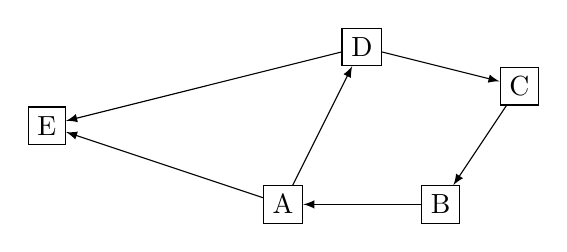
\begin{tikzpicture}
            \node[draw] (A) at (0,0) {A};
            \node[draw] (B) at (2,0) {B};
            \node[draw] (C) at (3,1.5) {C};
            \node[draw] (D) at (1,2) {D};
            \node[draw] (E) at (-3,1) {E};
    
            \draw[->,>=latex] (B)--(A);
            \draw[->,>=latex] (A)--(E);
            \draw[->,>=latex] (D)--(E);
            \draw[->,>=latex] (A)--(D);
            \draw[->,>=latex] (D)--(C);
            \draw[->,>=latex] (C)--(B);
    
        \end{tikzpicture}
        \captionof{figure}{graphe orienté}
        \label{oriente}
    \end{center}

\end{frame}

\begin{frame}
    \frametitle{}
    \begin{center}
        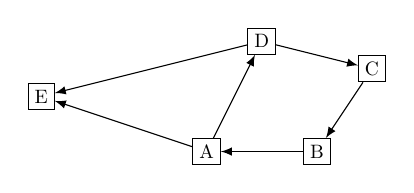
\begin{tikzpicture}[scale=0.7, transform shape]
            \node[draw] (A) at (0,0) {A};
            \node[draw] (B) at (2,0) {B};
            \node[draw] (C) at (3,1.5) {C};
            \node[draw] (D) at (1,2) {D};
            \node[draw] (E) at (-3,1) {E};
    
            \draw[->,>=latex] (B)--(A);
            \draw[->,>=latex] (A)--(E);
            \draw[->,>=latex] (D)--(E);
            \draw[->,>=latex] (A)--(D);
            \draw[->,>=latex] (D)--(C);
            \draw[->,>=latex] (C)--(B);
    
        \end{tikzpicture}
        \captionof{figure}{graphe orienté}
        \label{oriente}
    \end{center}
    \begin{aretenir}[]
        Pour chaque nœud on peut définir ses \textbf{prédécesseurs} et ses \textbf{successeurs}.

            
            \note[item]{Le nœud E ne possède pas de \emph{successeur}.}

    \end{aretenir}

\end{frame}

\begin{frame}
    \frametitle{}

    \begin{activite}
        \begin{enumerate}
            \item Établir la matrice d'adjacence du graphe figure \ref{oriente}.
            \item Établir le dictionnaire des successeurs du graphe figure \ref{oriente}.
            \item Déterminer un cycle dans le graphe.
        \end{enumerate}
    \end{activite}
\note{on peut faire dictionnaire des prédécesseurs}
\end{frame}

\begin{frame}[fragile]
    \frametitle{Correction}

    \begin{center}
        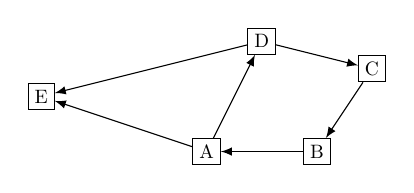
\begin{tikzpicture}[scale=0.7, transform shape]
            \node[draw] (A) at (0,0) {A};
            \node[draw] (B) at (2,0) {B};
            \node[draw] (C) at (3,1.5) {C};
            \node[draw] (D) at (1,2) {D};
            \node[draw] (E) at (-3,1) {E};
    
            \draw[->,>=latex] (B)--(A);
            \draw[->,>=latex] (A)--(E);
            \draw[->,>=latex] (D)--(E);
            \draw[->,>=latex] (A)--(D);
            \draw[->,>=latex] (D)--(C);
            \draw[->,>=latex] (C)--(B);
    
        \end{tikzpicture}
    \end{center}
    \begin{center}
    \begin{lstlisting}[language=Python]
matrice = [[0, 0, 0, 1, 1],
             [1, 0, 0, 0, 0],
             [0, 1, 0, 0, 0],
             [0, 0, 1, 0, 1],
             [0, 0, 0, 0, 0]]
    \end{lstlisting}
    \captionof{code}{Matrice d'adjacence}
    \end{center}
    \note{La matrice n'est plus symétrique}

\end{frame}

\begin{frame}[fragile]
    \frametitle{Correction}

    \begin{center}
        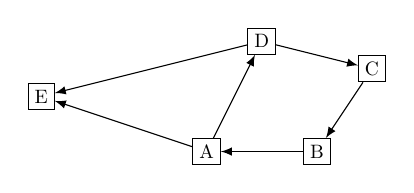
\begin{tikzpicture}[scale=0.7, transform shape]
            \node[draw] (A) at (0,0) {A};
            \node[draw] (B) at (2,0) {B};
            \node[draw] (C) at (3,1.5) {C};
            \node[draw] (D) at (1,2) {D};
            \node[draw] (E) at (-3,1) {E};
    
            \draw[->,>=latex] (B)--(A);
            \draw[->,>=latex] (A)--(E);
            \draw[->,>=latex] (D)--(E);
            \draw[->,>=latex] (A)--(D);
            \draw[->,>=latex] (D)--(C);
            \draw[->,>=latex] (C)--(B);
    
        \end{tikzpicture}
    \end{center}
    \begin{center}
    \begin{lstlisting}[language=Python]
dico = {"A": {"D", "E"},
          "B": {"A"},
          "C": {"B"},
          "D": {"C", "E"},
          "E": set()}
    \end{lstlisting}
    \captionof{code}{Dictionnaire d'adjacence}
    \end{center}
    \note{On peut utiliser des tableaux en place des ensembles.}

\end{frame}

\begin{frame}[fragile]
    \frametitle{Correction}

    \begin{center}
        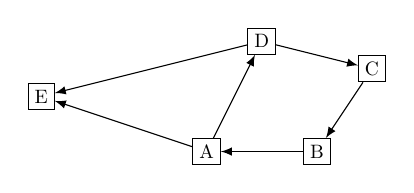
\begin{tikzpicture}[scale=0.7, transform shape]
            \node[draw] (A) at (0,0) {A};
            \node[draw] (B) at (2,0) {B};
            \node[draw] (C) at (3,1.5) {C};
            \node[draw] (D) at (1,2) {D};
            \node[draw] (E) at (-3,1) {E};
    
            \draw[->,>=latex] (B)--(A);
            \draw[->,>=latex] (A)--(E);
            \draw[->,>=latex] (D)--(E);
            \draw[->,>=latex] (A)--(D);
            \draw[->,>=latex] (D)--(C);
            \draw[->,>=latex] (C)--(B);
    
        \end{tikzpicture}
    \end{center}
    \begin{center}
    {\LARGE A $\rightarrow$ D $\rightarrow$ C $\rightarrow$ B $\rightarrow$ A}
    \end{center}

\end{frame}
\subsection{Graphe pondéré}
\begin{frame}
    \frametitle{}

    \begin{center}
        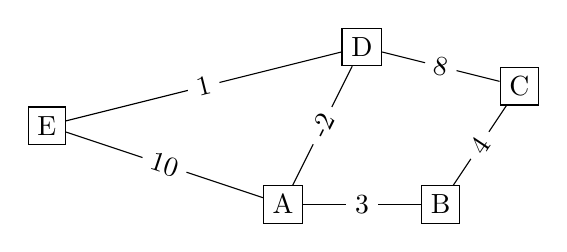
\begin{tikzpicture}
            \node[draw] (A) at (0,0) {A};
            \node[draw] (B) at (2,0) {B};
            \node[draw] (C) at (3,1.5) {C};
            \node[draw] (D) at (1,2) {D};
            \node[draw] (E) at (-3,1) {E};
    
            \draw (A)--(B) node[sloped, midway, fill=white]{3};
            \draw (A)--(E) node[sloped, midway, fill=white]{10};
            \draw (D)--(E) node[sloped, midway, fill=white]{1};
            \draw (A)--(D) node[sloped, midway, fill=white]{-2};
            \draw (D)--(C) node[sloped, midway, fill=white]{8};
            \draw (C)--(B) node[sloped, midway, fill=white]{4};
    
        \end{tikzpicture}
        \captionof{figure}{graphe non orienté pondéré}
        \label{pondere}
    \end{center}

    \note{pondération peut être négative}
\end{frame}

\begin{frame}
    \frametitle{}

    \begin{activite}
        \begin{enumerate}
            \item Établir la matrice d'adjacence du graphe figure \ref{pondere}.
            \item Établir le dictionnaire d'adjacence du graphe figure \ref{pondere}.
        \end{enumerate}
    \end{activite}

\end{frame}

\begin{frame}[fragile]
    \frametitle{Correction}

    \begin{center}
        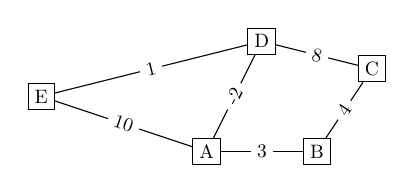
\begin{tikzpicture}[scale=0.7, transform shape]
            \node[draw] (A) at (0,0) {A};
            \node[draw] (B) at (2,0) {B};
            \node[draw] (C) at (3,1.5) {C};
            \node[draw] (D) at (1,2) {D};
            \node[draw] (E) at (-3,1) {E};
    
            \draw (A)--(B) node[sloped, midway, fill=white]{3};
            \draw (A)--(E) node[sloped, midway, fill=white]{10};
            \draw (D)--(E) node[sloped, midway, fill=white]{1};
            \draw (A)--(D) node[sloped, midway, fill=white]{-2};
            \draw (D)--(C) node[sloped, midway, fill=white]{8};
            \draw (C)--(B) node[sloped, midway, fill=white]{4};
        \end{tikzpicture}
    \end{center}
    \begin{center}
    \begin{lstlisting}[language=Python]
matrice = [[0, 3, 0, -2, 10],
             [3, 0, 4, 0, 0],
             [0, 4, 0, 8, 0],
             [-2, 0, 8, 0, 1],
             [10, 0, 0, 1, 0]]
    \end{lstlisting}
    \captionof{code}{Matrice d'adjacence}
    \end{center}
    \note{La matrice est symétrique}

\end{frame}

\begin{frame}[fragile]
    \frametitle{Correction}

    \begin{center}
        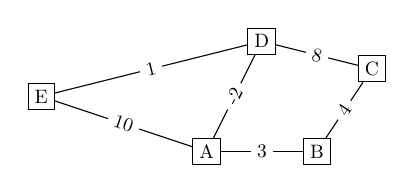
\begin{tikzpicture}[scale=0.7, transform shape]
            \node[draw] (A) at (0,0) {A};
            \node[draw] (B) at (2,0) {B};
            \node[draw] (C) at (3,1.5) {C};
            \node[draw] (D) at (1,2) {D};
            \node[draw] (E) at (-3,1) {E};
    
            \draw (A)--(B) node[sloped, midway, fill=white]{3};
            \draw (A)--(E) node[sloped, midway, fill=white]{10};
            \draw (D)--(E) node[sloped, midway, fill=white]{1};
            \draw (A)--(D) node[sloped, midway, fill=white]{-2};
            \draw (D)--(C) node[sloped, midway, fill=white]{8};
            \draw (C)--(B) node[sloped, midway, fill=white]{4};
        \end{tikzpicture}
    \end{center}
    \begin{center}
    \begin{lstlisting}[language=Python]
        dico = {"A": {"B": 3, "D": -2, "E": 10},
        "B": {"A": 3, "C": 4},
        "C": {"B": 4, "D": 8},
        "D": {"A": -2, "C": 8, "E": 1},
        "E": {"D": 1, "E": 10}}
    \end{lstlisting}
    \captionof{code}{Dictionnaire d'adjacence}
    \end{center}
    \note{Dictionnaire de dictionnaires}

\end{frame}

\section{Protocole RIP: algorithme de Bellman-Ford}
\subsection{Principe}
\begin{frame}
    \frametitle{Algorithme de Bellman-Ford: Fin des années 50}

    \begin{center}
        \emph{La distance pour atteindre chaque nœud correspond à la distance pour atteindre son prédécesseur à laquelle on ajoute le poids de l'arête les séparant.}
    \end{center}

\end{frame}

\begin{frame}
    \frametitle{Démarche récursive}
\note[item]{Bellman \guill{père de l'approche dynamique}}
\note[item]{\begin{aretenir}[Remarque]
    Dans le graphe figure \ref{rip} les pondérations représentent un nombre de routeurs traversés pour atteindre le nœud (routeur) suivant.
\end{aretenir}}
\begin{center}
    \begin{tikzpicture}
        \node[draw] (A) at (0,0) {A};
        \node[draw] (B) at (3,0) {B};
        \node[draw] (C) at (6,0) {C};
        \node[draw] (D) at (9,0) {D};
        \node[draw] (E) at (6,-2) {E};
        \node[draw] (F) at (6,2) {F};

        \draw[->,>=latex] (A)--(B) node[sloped, midway, fill=white]{2};
        %\draw[->,>=latex] (B)--(C) node[sloped, midway, fill=white]{6};
        \draw[->,>=latex] (C)--(D) node[sloped, midway, fill=white]{2};
        \draw[->,>=latex] (A)--(F) node[sloped, midway, fill=white]{3};
        \draw[->,>=latex] (B)--(E) node[sloped, midway, fill=white]{4};
        \draw[->,>=latex] (F)--(C) node[sloped, midway, fill=white]{2};
        \draw[->,>=latex] (E)--(C) node[sloped, midway, fill=white]{1};
        \draw[->,>=latex] (E)--(D) node[sloped, midway, fill=white]{5};
        \draw[->,>=latex] (D)--(F) node[sloped, midway, fill=white]{2};

    \end{tikzpicture}
    \captionof{figure}{graphe orienté pondéré}
    \label{rip}
\end{center}
\begin{center}
    En pratique nous allons utiliser une approche itérative \emph{bottom-up}.
\end{center}
\end{frame}

\begin{frame}
    \frametitle{Pour chaque routeur}

    On obtient un tableau contenant la distance minimale entre le routeur de départ et chaque autre routeur.
    \note{peut servir pour retrouver chemin, distance mini\dots}

\end{frame}


\subsection{Mise en application}
\begin{frame}[fragile]
    \frametitle{}

    \begin{center}
        \begin{lstlisting}[language=Bash, basicstyle=\small, xrightmargin=0.5em, xleftmargin=0.5em]
Créer un tableau des distances entre A et les routeurs (A inclus), initialisées à l'infini.
Dans le tableau modifier la distance vers A à 0.

Tant que (le nombre d'itérations) < (nombre de routeurs)
    Pour chaque arc du graphe
        Si (la distance du routeur) > (la distance de son prédécesseur + poids de l'arc entre les deux routeurs)
            La distance du routeur est remplacée par cette nouvelle valeur
    \end{lstlisting}
        \captionof{code}{Algorithme de Bellman Ford}
        \label{bf}
    \end{center}
\note[item]{ligne 2 de l'algo: en effet distance de A à A = 0}
\note[item]{ligne 4: on fait autant d'itérations qu'il y a de routeurs = pire des cas $\rightarrow$ on pourra améliorer}
\end{frame}

\begin{frame}
    \frametitle{Initialisation}

    \begin{center}
        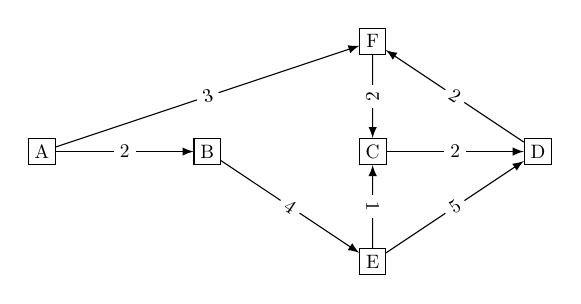
\begin{tikzpicture}[scale=0.7, transform shape]
            \node[draw] (A) at (0,0) {A};
            \node[draw] (B) at (3,0) {B};
            \node[draw] (C) at (6,0) {C};
            \node[draw] (D) at (9,0) {D};
            \node[draw] (E) at (6,-2) {E};
            \node[draw] (F) at (6,2) {F};
    
            \draw[->,>=latex] (A)--(B) node[sloped, midway, fill=white]{2};
            %\draw[->,>=latex] (B)--(C) node[sloped, midway, fill=white]{6};
            \draw[->,>=latex] (C)--(D) node[sloped, midway, fill=white]{2};
            \draw[->,>=latex] (A)--(F) node[sloped, midway, fill=white]{3};
            \draw[->,>=latex] (B)--(E) node[sloped, midway, fill=white]{4};
            \draw[->,>=latex] (F)--(C) node[sloped, midway, fill=white]{2};
            \draw[->,>=latex] (E)--(C) node[sloped, midway, fill=white]{1};
            \draw[->,>=latex] (E)--(D) node[sloped, midway, fill=white]{5};
            \draw[->,>=latex] (D)--(F) node[sloped, midway, fill=white]{2};
    
        \end{tikzpicture}
    \end{center}
    \begin{center}
        \begin{tabular}{|*{6}{c|}}
            \hline
            A & B      & C      & D      & E      & F      \\
            \hline
            0 & \infty & \infty & \infty & \infty & \infty \\
            \hline
        \end{tabular}
    \end{center}
\end{frame}

\begin{frame}
    \frametitle{Première itération}

    \begin{center}
        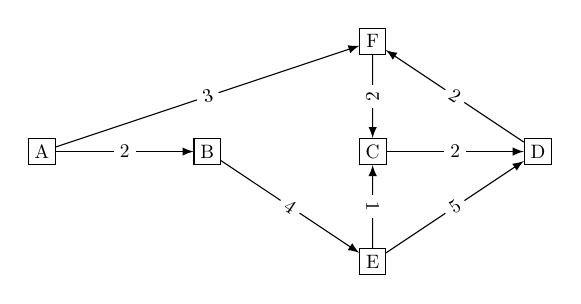
\begin{tikzpicture}[scale=0.7, transform shape]
            \node[draw] (A) at (0,0) {A};
            \node[draw] (B) at (3,0) {B};
            \node[draw] (C) at (6,0) {C};
            \node[draw] (D) at (9,0) {D};
            \node[draw] (E) at (6,-2) {E};
            \node[draw] (F) at (6,2) {F};
    
            \draw[->,>=latex] (A)--(B) node[sloped, midway, fill=white]{2};
            %\draw[->,>=latex] (B)--(C) node[sloped, midway, fill=white]{6};
            \draw[->,>=latex] (C)--(D) node[sloped, midway, fill=white]{2};
            \draw[->,>=latex] (A)--(F) node[sloped, midway, fill=white]{3};
            \draw[->,>=latex] (B)--(E) node[sloped, midway, fill=white]{4};
            \draw[->,>=latex] (F)--(C) node[sloped, midway, fill=white]{2};
            \draw[->,>=latex] (E)--(C) node[sloped, midway, fill=white]{1};
            \draw[->,>=latex] (E)--(D) node[sloped, midway, fill=white]{5};
            \draw[->,>=latex] (D)--(F) node[sloped, midway, fill=white]{2};
    
        \end{tikzpicture}
    \end{center}
    \begin{center}
        \begin{tabular}{|*{6}{c|}}
            \hline
            A & B      & C      & D      & E      & F      \\
            \hline
            0 & \textbf{2 (A)} & \infty & \infty & \infty & \infty \\
            \hline
        \end{tabular}
    \end{center}
    \note{La distance calculée pour atteindre B correspond à la distance (du tableau) de son prédécesseur (A) augmentée du poids de l'arc A-B:
    $$0+2 = 2 < \infty$$}
\end{frame}
\begin{frame}
    \frametitle{}

    \begin{activite}
        Continuer de dérouler l'algorithme sur le graphe figure \ref{rip}.
    \end{activite}

\end{frame}

\begin{frame}
    \frametitle{Première itération}

    \begin{center}
        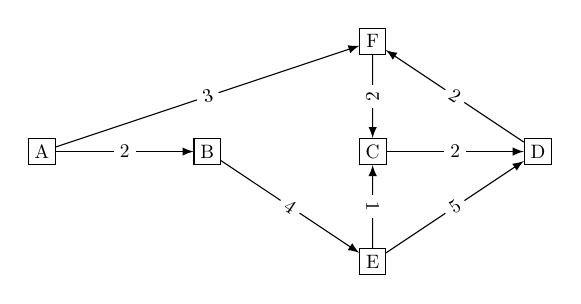
\begin{tikzpicture}[scale=0.7, transform shape]
            \node[draw] (A) at (0,0) {A};
            \node[draw] (B) at (3,0) {B};
            \node[draw] (C) at (6,0) {C};
            \node[draw] (D) at (9,0) {D};
            \node[draw] (E) at (6,-2) {E};
            \node[draw] (F) at (6,2) {F};
    
            \draw[->,>=latex] (A)--(B) node[sloped, midway, fill=white]{2};
            %\draw[->,>=latex] (B)--(C) node[sloped, midway, fill=white]{6};
            \draw[->,>=latex] (C)--(D) node[sloped, midway, fill=white]{2};
            \draw[->,>=latex] (A)--(F) node[sloped, midway, fill=white]{3};
            \draw[->,>=latex] (B)--(E) node[sloped, midway, fill=white]{4};
            \draw[->,>=latex] (F)--(C) node[sloped, midway, fill=white]{2};
            \draw[->,>=latex] (E)--(C) node[sloped, midway, fill=white]{1};
            \draw[->,>=latex] (E)--(D) node[sloped, midway, fill=white]{5};
            \draw[->,>=latex] (D)--(F) node[sloped, midway, fill=white]{2};
    
        \end{tikzpicture}
    \end{center}
    \begin{center}
        \begin{tabular}{|*{6}{c|}}
            \hline
            A & B      & C      & D      & E      & F      \\
            \hline
            0 & 2 (A) & \infty & \infty & \infty & \infty \\
            \hline
        \end{tabular}
    \end{center}
    Premier prédécesseur de C: E
    $$\infty+1 = \infty \nless \infty$$
    \note{On est toujours dans la première itération; on vérifie chaque arc.}
\end{frame}

\begin{frame}
    \frametitle{Première itération}

    \begin{center}
        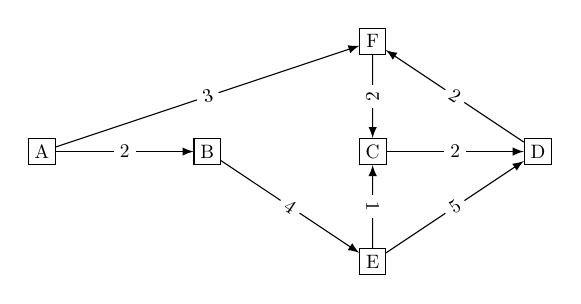
\begin{tikzpicture}[scale=0.7, transform shape]
            \node[draw] (A) at (0,0) {A};
            \node[draw] (B) at (3,0) {B};
            \node[draw] (C) at (6,0) {C};
            \node[draw] (D) at (9,0) {D};
            \node[draw] (E) at (6,-2) {E};
            \node[draw] (F) at (6,2) {F};
    
            \draw[->,>=latex] (A)--(B) node[sloped, midway, fill=white]{2};
            %\draw[->,>=latex] (B)--(C) node[sloped, midway, fill=white]{6};
            \draw[->,>=latex] (C)--(D) node[sloped, midway, fill=white]{2};
            \draw[->,>=latex] (A)--(F) node[sloped, midway, fill=white]{3};
            \draw[->,>=latex] (B)--(E) node[sloped, midway, fill=white]{4};
            \draw[->,>=latex] (F)--(C) node[sloped, midway, fill=white]{2};
            \draw[->,>=latex] (E)--(C) node[sloped, midway, fill=white]{1};
            \draw[->,>=latex] (E)--(D) node[sloped, midway, fill=white]{5};
            \draw[->,>=latex] (D)--(F) node[sloped, midway, fill=white]{2};
    
        \end{tikzpicture}
    \end{center}
    \begin{center}
        \begin{tabular}{|*{6}{c|}}
            \hline
            A & B      & C      & D      & E      & F      \\
            \hline
            0 & 2 (A) & \infty & \infty & \infty & \infty \\
            \hline
        \end{tabular}
    \end{center}
    Second prédécesseur de C: F
    $$\infty+2 = \infty \nless  \infty$$
\end{frame}

\begin{frame}
    \frametitle{Première itération}

    \begin{center}
        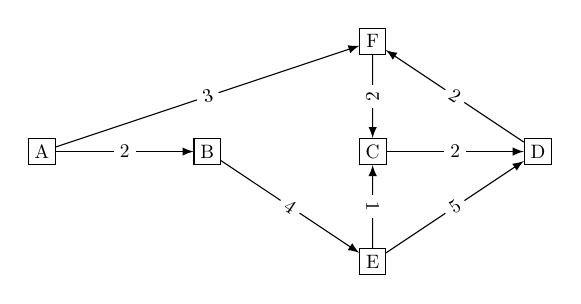
\begin{tikzpicture}[scale=0.7, transform shape]
            \node[draw] (A) at (0,0) {A};
            \node[draw] (B) at (3,0) {B};
            \node[draw] (C) at (6,0) {C};
            \node[draw] (D) at (9,0) {D};
            \node[draw] (E) at (6,-2) {E};
            \node[draw] (F) at (6,2) {F};
    
            \draw[->,>=latex] (A)--(B) node[sloped, midway, fill=white]{2};
            %\draw[->,>=latex] (B)--(C) node[sloped, midway, fill=white]{6};
            \draw[->,>=latex] (C)--(D) node[sloped, midway, fill=white]{2};
            \draw[->,>=latex] (A)--(F) node[sloped, midway, fill=white]{3};
            \draw[->,>=latex] (B)--(E) node[sloped, midway, fill=white]{4};
            \draw[->,>=latex] (F)--(C) node[sloped, midway, fill=white]{2};
            \draw[->,>=latex] (E)--(C) node[sloped, midway, fill=white]{1};
            \draw[->,>=latex] (E)--(D) node[sloped, midway, fill=white]{5};
            \draw[->,>=latex] (D)--(F) node[sloped, midway, fill=white]{2};
    
        \end{tikzpicture}
    \end{center}
    \begin{center}
        \begin{tabular}{|*{6}{c|}}
            \hline
            A & B      & C      & D      & E      & F      \\
            \hline
            0 & 2 (A) & \infty & \infty & \infty & \infty \\
            \hline
        \end{tabular}
    \end{center}
    Même constat pour D
\end{frame}

\begin{frame}
    \frametitle{Première itération}

    \begin{center}
        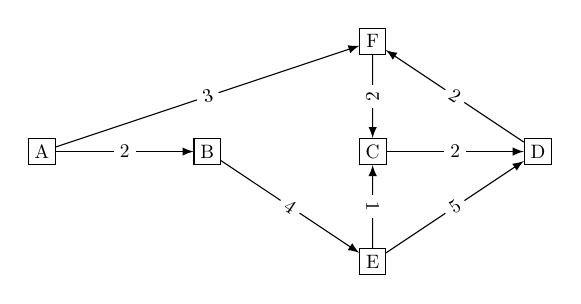
\begin{tikzpicture}[scale=0.7, transform shape]
            \node[draw] (A) at (0,0) {A};
            \node[draw] (B) at (3,0) {B};
            \node[draw] (C) at (6,0) {C};
            \node[draw] (D) at (9,0) {D};
            \node[draw] (E) at (6,-2) {E};
            \node[draw] (F) at (6,2) {F};
    
            \draw[->,>=latex] (A)--(B) node[sloped, midway, fill=white]{2};
            %\draw[->,>=latex] (B)--(C) node[sloped, midway, fill=white]{6};
            \draw[->,>=latex] (C)--(D) node[sloped, midway, fill=white]{2};
            \draw[->,>=latex] (A)--(F) node[sloped, midway, fill=white]{3};
            \draw[->,>=latex] (B)--(E) node[sloped, midway, fill=white]{4};
            \draw[->,>=latex] (F)--(C) node[sloped, midway, fill=white]{2};
            \draw[->,>=latex] (E)--(C) node[sloped, midway, fill=white]{1};
            \draw[->,>=latex] (E)--(D) node[sloped, midway, fill=white]{5};
            \draw[->,>=latex] (D)--(F) node[sloped, midway, fill=white]{2};
    
        \end{tikzpicture}
    \end{center}
    \begin{center}
        \begin{tabular}{|*{6}{c|}}
            \hline
            A & B      & C      & D      & E      & F      \\
            \hline
            0 & 2 (A) & \infty & \infty & \textbf{6 (B)} & \infty \\
            \hline
        \end{tabular}
    \end{center}
    Prédécesseur de E: B
    $$2+4 = 6 <  \infty$$
\end{frame}

\begin{frame}
    \frametitle{Première itération}

    \begin{center}
        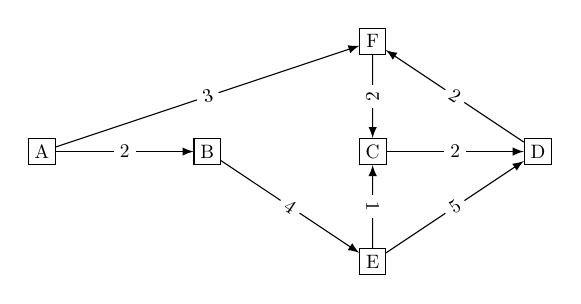
\begin{tikzpicture}[scale=0.7, transform shape]
            \node[draw] (A) at (0,0) {A};
            \node[draw] (B) at (3,0) {B};
            \node[draw] (C) at (6,0) {C};
            \node[draw] (D) at (9,0) {D};
            \node[draw] (E) at (6,-2) {E};
            \node[draw] (F) at (6,2) {F};
    
            \draw[->,>=latex] (A)--(B) node[sloped, midway, fill=white]{2};
            %\draw[->,>=latex] (B)--(C) node[sloped, midway, fill=white]{6};
            \draw[->,>=latex] (C)--(D) node[sloped, midway, fill=white]{2};
            \draw[->,>=latex] (A)--(F) node[sloped, midway, fill=white]{3};
            \draw[->,>=latex] (B)--(E) node[sloped, midway, fill=white]{4};
            \draw[->,>=latex] (F)--(C) node[sloped, midway, fill=white]{2};
            \draw[->,>=latex] (E)--(C) node[sloped, midway, fill=white]{1};
            \draw[->,>=latex] (E)--(D) node[sloped, midway, fill=white]{5};
            \draw[->,>=latex] (D)--(F) node[sloped, midway, fill=white]{2};
    
        \end{tikzpicture}
    \end{center}
    \begin{center}
        \begin{tabular}{|*{6}{c|}}
            \hline
            A & B      & C      & D      & E      & F      \\
            \hline
            0 & 2 (A)& \infty & \infty & 6 (B) & \textbf{3 (A)}  \\
            \hline
        \end{tabular}
    \end{center}
    Premier prédécesseur de F: A
    $$0+3 = 3 <  \infty$$
\end{frame}

\begin{frame}
    \frametitle{Première itération}

    \begin{center}
        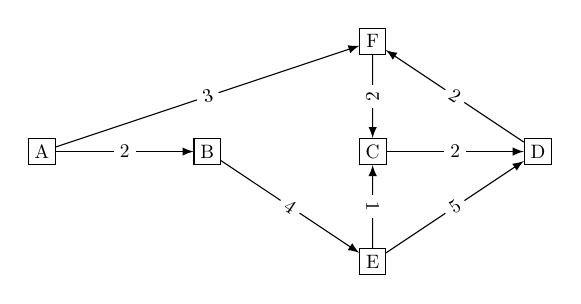
\begin{tikzpicture}[scale=0.7, transform shape]
            \node[draw] (A) at (0,0) {A};
            \node[draw] (B) at (3,0) {B};
            \node[draw] (C) at (6,0) {C};
            \node[draw] (D) at (9,0) {D};
            \node[draw] (E) at (6,-2) {E};
            \node[draw] (F) at (6,2) {F};
    
            \draw[->,>=latex] (A)--(B) node[sloped, midway, fill=white]{2};
            %\draw[->,>=latex] (B)--(C) node[sloped, midway, fill=white]{6};
            \draw[->,>=latex] (C)--(D) node[sloped, midway, fill=white]{2};
            \draw[->,>=latex] (A)--(F) node[sloped, midway, fill=white]{3};
            \draw[->,>=latex] (B)--(E) node[sloped, midway, fill=white]{4};
            \draw[->,>=latex] (F)--(C) node[sloped, midway, fill=white]{2};
            \draw[->,>=latex] (E)--(C) node[sloped, midway, fill=white]{1};
            \draw[->,>=latex] (E)--(D) node[sloped, midway, fill=white]{5};
            \draw[->,>=latex] (D)--(F) node[sloped, midway, fill=white]{2};
    
        \end{tikzpicture}
    \end{center}
    \begin{center}
        \begin{tabular}{|*{6}{c|}}
            \hline
            A & B      & C      & D      & E      & F      \\
            \hline
            0 & 2 (A)& \infty & \infty & 6 (B) & 3 (A) \\
            \hline
        \end{tabular}
    \end{center}
    Second prédécesseur de F: D
    $$\infty+2 = \infty \nless  3$$
\end{frame}

\begin{frame}
    \frametitle{Première itération}

    \begin{center}
        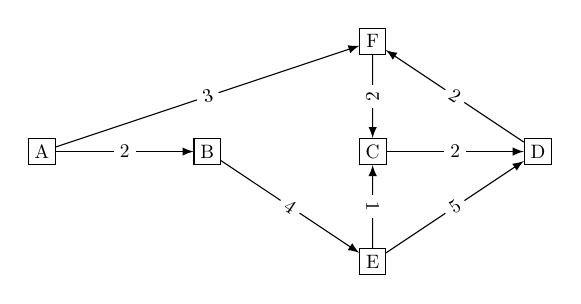
\begin{tikzpicture}[scale=0.7, transform shape]
            \node[draw] (A) at (0,0) {A};
            \node[draw] (B) at (3,0) {B};
            \node[draw] (C) at (6,0) {C};
            \node[draw] (D) at (9,0) {D};
            \node[draw] (E) at (6,-2) {E};
            \node[draw] (F) at (6,2) {F};
    
            \draw[->,>=latex] (A)--(B) node[sloped, midway, fill=white]{2};
            %\draw[->,>=latex] (B)--(C) node[sloped, midway, fill=white]{6};
            \draw[->,>=latex] (C)--(D) node[sloped, midway, fill=white]{2};
            \draw[->,>=latex] (A)--(F) node[sloped, midway, fill=white]{3};
            \draw[->,>=latex] (B)--(E) node[sloped, midway, fill=white]{4};
            \draw[->,>=latex] (F)--(C) node[sloped, midway, fill=white]{2};
            \draw[->,>=latex] (E)--(C) node[sloped, midway, fill=white]{1};
            \draw[->,>=latex] (E)--(D) node[sloped, midway, fill=white]{5};
            \draw[->,>=latex] (D)--(F) node[sloped, midway, fill=white]{2};
    
        \end{tikzpicture}
    \end{center}
    \begin{center}
        \begin{tabular}{|*{6}{c|}}
            \hline
            A & B      & C      & D      & E      & F      \\
            \hline
            0 & 2 (A) & \infty & \infty & 6 (B) & 3 (A) \\
            \hline
        \end{tabular}
    \end{center}
    \begin{center}
        {\LARGE Fin de la première itération}
    \end{center}
\end{frame}

\begin{frame}
    \frametitle{Deuxième itération}

    \begin{center}
        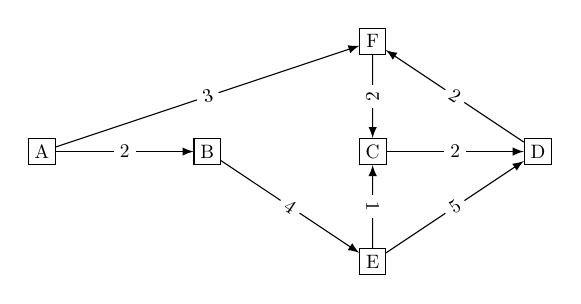
\begin{tikzpicture}[scale=0.7, transform shape]
            \node[draw] (A) at (0,0) {A};
            \node[draw] (B) at (3,0) {B};
            \node[draw] (C) at (6,0) {C};
            \node[draw] (D) at (9,0) {D};
            \node[draw] (E) at (6,-2) {E};
            \node[draw] (F) at (6,2) {F};
    
            \draw[->,>=latex] (A)--(B) node[sloped, midway, fill=white]{2};
            %\draw[->,>=latex] (B)--(C) node[sloped, midway, fill=white]{6};
            \draw[->,>=latex] (C)--(D) node[sloped, midway, fill=white]{2};
            \draw[->,>=latex] (A)--(F) node[sloped, midway, fill=white]{3};
            \draw[->,>=latex] (B)--(E) node[sloped, midway, fill=white]{4};
            \draw[->,>=latex] (F)--(C) node[sloped, midway, fill=white]{2};
            \draw[->,>=latex] (E)--(C) node[sloped, midway, fill=white]{1};
            \draw[->,>=latex] (E)--(D) node[sloped, midway, fill=white]{5};
            \draw[->,>=latex] (D)--(F) node[sloped, midway, fill=white]{2};
    
        \end{tikzpicture}
    \end{center}
    \begin{center}
        \begin{tabular}{|*{6}{c|}}
            \hline
            A & B      & C      & D      & E      & F      \\
            \hline
            0 & 2 (A) & \infty & \infty & 6 (B) & 3 (A) \\
            \hline
            0 & 2 (A) & \infty & \infty & 6 (B) & 3 (A) \\
            \hline
        \end{tabular}
    \end{center}
    {\Large Pas de modification pour A et B}
\end{frame}

\begin{frame}
    \frametitle{Deuxième itération}

    \begin{center}
        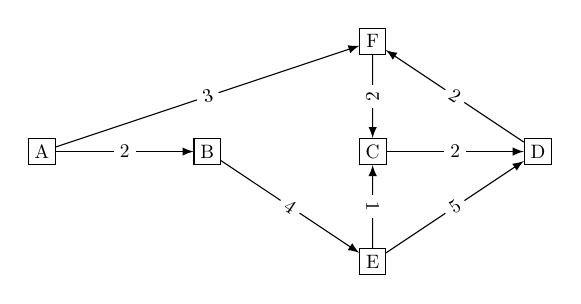
\begin{tikzpicture}[scale=0.7, transform shape]
            \node[draw] (A) at (0,0) {A};
            \node[draw] (B) at (3,0) {B};
            \node[draw] (C) at (6,0) {C};
            \node[draw] (D) at (9,0) {D};
            \node[draw] (E) at (6,-2) {E};
            \node[draw] (F) at (6,2) {F};
    
            \draw[->,>=latex] (A)--(B) node[sloped, midway, fill=white]{2};
            %\draw[->,>=latex] (B)--(C) node[sloped, midway, fill=white]{6};
            \draw[->,>=latex] (C)--(D) node[sloped, midway, fill=white]{2};
            \draw[->,>=latex] (A)--(F) node[sloped, midway, fill=white]{3};
            \draw[->,>=latex] (B)--(E) node[sloped, midway, fill=white]{4};
            \draw[->,>=latex] (F)--(C) node[sloped, midway, fill=white]{2};
            \draw[->,>=latex] (E)--(C) node[sloped, midway, fill=white]{1};
            \draw[->,>=latex] (E)--(D) node[sloped, midway, fill=white]{5};
            \draw[->,>=latex] (D)--(F) node[sloped, midway, fill=white]{2};
    
        \end{tikzpicture}
    \end{center}
    \begin{center}
        \begin{tabular}{|*{6}{c|}}
            \hline
            A & B      & C      & D      & E      & F      \\
            \hline
            0 & 2 (A) & \infty & \infty & 6 (B) & 3 (A) \\
            \hline
            0 & 2 (A) & \textbf{7 (E)} & \infty & 6 (B)& 3 (A)\\
            \hline
        \end{tabular}
    \end{center}
    Premier prédécesseur de C: E
    $$6+1 = 7 < \infty$$
    
\end{frame}

\begin{frame}
    \frametitle{Deuxième itération}

    \begin{center}
        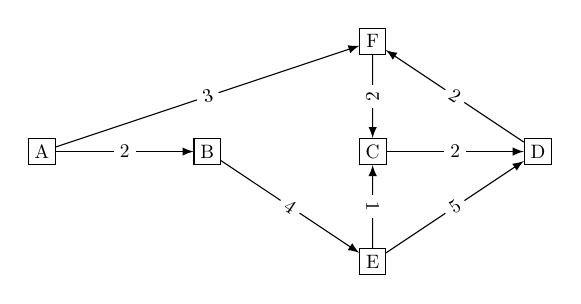
\begin{tikzpicture}[scale=0.7, transform shape]
            \node[draw] (A) at (0,0) {A};
            \node[draw] (B) at (3,0) {B};
            \node[draw] (C) at (6,0) {C};
            \node[draw] (D) at (9,0) {D};
            \node[draw] (E) at (6,-2) {E};
            \node[draw] (F) at (6,2) {F};
    
            \draw[->,>=latex] (A)--(B) node[sloped, midway, fill=white]{2};
            %\draw[->,>=latex] (B)--(C) node[sloped, midway, fill=white]{6};
            \draw[->,>=latex] (C)--(D) node[sloped, midway, fill=white]{2};
            \draw[->,>=latex] (A)--(F) node[sloped, midway, fill=white]{3};
            \draw[->,>=latex] (B)--(E) node[sloped, midway, fill=white]{4};
            \draw[->,>=latex] (F)--(C) node[sloped, midway, fill=white]{2};
            \draw[->,>=latex] (E)--(C) node[sloped, midway, fill=white]{1};
            \draw[->,>=latex] (E)--(D) node[sloped, midway, fill=white]{5};
            \draw[->,>=latex] (D)--(F) node[sloped, midway, fill=white]{2};
    
        \end{tikzpicture}
    \end{center}
    \begin{center}
        \begin{tabular}{|*{6}{c|}}
            \hline
            A & B      & C      & D      & E      & F      \\
            \hline
            0 & 2 (A) & \infty & \infty & 6 (B) & 3 (A) \\
            \hline
            0 & 2 (A) & \textbf{5 (F)} & \infty & 6 (B) & 3 (A) \\
            \hline
        \end{tabular}
    \end{center}
    Second prédécesseur de C: F
    $$3+2 = 5 < 7$$
    
\end{frame}

\begin{frame}
    \frametitle{Deuxième itération}

    \begin{center}
        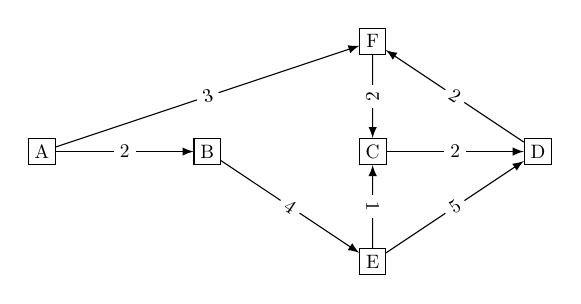
\begin{tikzpicture}[scale=0.7, transform shape]
            \node[draw] (A) at (0,0) {A};
            \node[draw] (B) at (3,0) {B};
            \node[draw] (C) at (6,0) {C};
            \node[draw] (D) at (9,0) {D};
            \node[draw] (E) at (6,-2) {E};
            \node[draw] (F) at (6,2) {F};
    
            \draw[->,>=latex] (A)--(B) node[sloped, midway, fill=white]{2};
            %\draw[->,>=latex] (B)--(C) node[sloped, midway, fill=white]{6};
            \draw[->,>=latex] (C)--(D) node[sloped, midway, fill=white]{2};
            \draw[->,>=latex] (A)--(F) node[sloped, midway, fill=white]{3};
            \draw[->,>=latex] (B)--(E) node[sloped, midway, fill=white]{4};
            \draw[->,>=latex] (F)--(C) node[sloped, midway, fill=white]{2};
            \draw[->,>=latex] (E)--(C) node[sloped, midway, fill=white]{1};
            \draw[->,>=latex] (E)--(D) node[sloped, midway, fill=white]{5};
            \draw[->,>=latex] (D)--(F) node[sloped, midway, fill=white]{2};
    
        \end{tikzpicture}
    \end{center}
    \begin{center}
        \begin{tabular}{|*{6}{c|}}
            \hline
            A & B      & C      & D      & E      & F      \\
            \hline
            0 & 2 (A) & \infty & \infty & 6 (B) & 3 (A) \\
            \hline
            0 & 2 (A) & 5 (F) & \textbf{7 (C)} & 6 (B) & 3 (A) \\
            \hline
        \end{tabular}
    \end{center}
    Premier prédécesseur de D: C
    $$5+2 = 7 < \infty$$
    
\end{frame}

\begin{frame}
    \frametitle{Deuxième itération}

    \begin{center}
        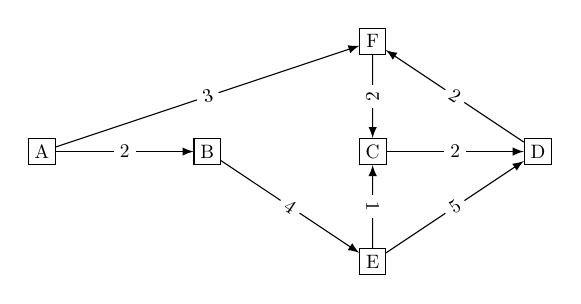
\begin{tikzpicture}[scale=0.7, transform shape]
            \node[draw] (A) at (0,0) {A};
            \node[draw] (B) at (3,0) {B};
            \node[draw] (C) at (6,0) {C};
            \node[draw] (D) at (9,0) {D};
            \node[draw] (E) at (6,-2) {E};
            \node[draw] (F) at (6,2) {F};
    
            \draw[->,>=latex] (A)--(B) node[sloped, midway, fill=white]{2};
            %\draw[->,>=latex] (B)--(C) node[sloped, midway, fill=white]{6};
            \draw[->,>=latex] (C)--(D) node[sloped, midway, fill=white]{2};
            \draw[->,>=latex] (A)--(F) node[sloped, midway, fill=white]{3};
            \draw[->,>=latex] (B)--(E) node[sloped, midway, fill=white]{4};
            \draw[->,>=latex] (F)--(C) node[sloped, midway, fill=white]{2};
            \draw[->,>=latex] (E)--(C) node[sloped, midway, fill=white]{1};
            \draw[->,>=latex] (E)--(D) node[sloped, midway, fill=white]{5};
            \draw[->,>=latex] (D)--(F) node[sloped, midway, fill=white]{2};
    
        \end{tikzpicture}
    \end{center}
    \begin{center}
        \begin{tabular}{|*{6}{c|}}
            \hline
            A & B      & C      & D      & E      & F      \\
            \hline
            0 & 2 (A) & \infty & \infty & 6 (B) & 3 (A) \\
            \hline
            0 & 2 (A) & 5 (F) & 7 (C) & 6 (B) & 3 (A) \\
            \hline
        \end{tabular}
    \end{center}
    Second prédécesseur de D: E
    $$6+5 = 11 \nless 7$$
    
\end{frame}
\begin{frame}
    \frametitle{Deuxième itération}

    \begin{center}
        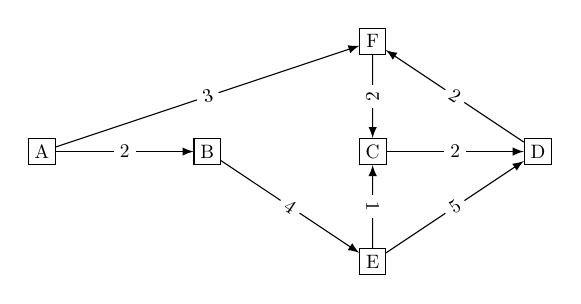
\begin{tikzpicture}[scale=0.7, transform shape]
            \node[draw] (A) at (0,0) {A};
            \node[draw] (B) at (3,0) {B};
            \node[draw] (C) at (6,0) {C};
            \node[draw] (D) at (9,0) {D};
            \node[draw] (E) at (6,-2) {E};
            \node[draw] (F) at (6,2) {F};
    
            \draw[->,>=latex] (A)--(B) node[sloped, midway, fill=white]{2};
            %\draw[->,>=latex] (B)--(C) node[sloped, midway, fill=white]{6};
            \draw[->,>=latex] (C)--(D) node[sloped, midway, fill=white]{2};
            \draw[->,>=latex] (A)--(F) node[sloped, midway, fill=white]{3};
            \draw[->,>=latex] (B)--(E) node[sloped, midway, fill=white]{4};
            \draw[->,>=latex] (F)--(C) node[sloped, midway, fill=white]{2};
            \draw[->,>=latex] (E)--(C) node[sloped, midway, fill=white]{1};
            \draw[->,>=latex] (E)--(D) node[sloped, midway, fill=white]{5};
            \draw[->,>=latex] (D)--(F) node[sloped, midway, fill=white]{2};
    
        \end{tikzpicture}
    \end{center}
    \begin{center}
        \begin{tabular}{|*{6}{c|}}
            \hline
            A & B      & C      & D      & E      & F      \\
            \hline
            0 & 2 (A) & \infty & \infty & 6 (B) & 3 (A) \\
            \hline
            0 & 2 (A) & 5 (F) & 7 (C) & 6 (B) & 3 (A) \\
            \hline
        \end{tabular}
    \end{center}
    \begin{center}
        {\LARGE Pas de changement pour E et F}
    \end{center}
    
\end{frame}
\begin{frame}
    \frametitle{Deuxième itération}

    \begin{center}
        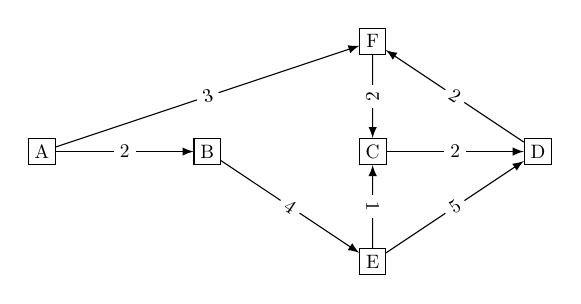
\begin{tikzpicture}[scale=0.7, transform shape]
            \node[draw] (A) at (0,0) {A};
            \node[draw] (B) at (3,0) {B};
            \node[draw] (C) at (6,0) {C};
            \node[draw] (D) at (9,0) {D};
            \node[draw] (E) at (6,-2) {E};
            \node[draw] (F) at (6,2) {F};
    
            \draw[->,>=latex] (A)--(B) node[sloped, midway, fill=white]{2};
            %\draw[->,>=latex] (B)--(C) node[sloped, midway, fill=white]{6};
            \draw[->,>=latex] (C)--(D) node[sloped, midway, fill=white]{2};
            \draw[->,>=latex] (A)--(F) node[sloped, midway, fill=white]{3};
            \draw[->,>=latex] (B)--(E) node[sloped, midway, fill=white]{4};
            \draw[->,>=latex] (F)--(C) node[sloped, midway, fill=white]{2};
            \draw[->,>=latex] (E)--(C) node[sloped, midway, fill=white]{1};
            \draw[->,>=latex] (E)--(D) node[sloped, midway, fill=white]{5};
            \draw[->,>=latex] (D)--(F) node[sloped, midway, fill=white]{2};
    
        \end{tikzpicture}
    \end{center}
    \begin{center}
        \begin{tabular}{|*{6}{c|}}
            \hline
            A & B      & C      & D      & E      & F      \\
            \hline
            0 & 2 (A) & \infty & \infty & 6 (B) & 3 (A) \\
            \hline
            0 & 2 (A) & 5 (F) & 7 (C) & 6 (B) & 3 (A) \\
            \hline
        \end{tabular}
    \end{center}
    \begin{center}
        {\LARGE Fin de la deuxième itération}
    \end{center}
    
\end{frame}

\begin{frame}
    \frametitle{Troisième itération}

    \begin{center}
        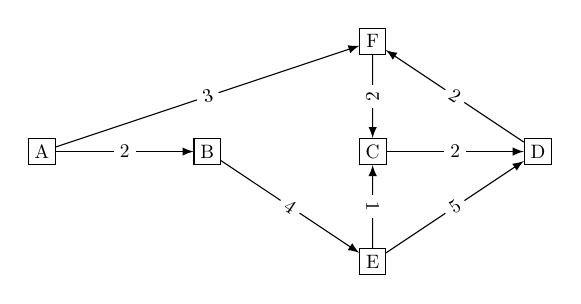
\begin{tikzpicture}[scale=0.7, transform shape]
            \node[draw] (A) at (0,0) {A};
            \node[draw] (B) at (3,0) {B};
            \node[draw] (C) at (6,0) {C};
            \node[draw] (D) at (9,0) {D};
            \node[draw] (E) at (6,-2) {E};
            \node[draw] (F) at (6,2) {F};
    
            \draw[->,>=latex] (A)--(B) node[sloped, midway, fill=white]{2};
            %\draw[->,>=latex] (B)--(C) node[sloped, midway, fill=white]{6};
            \draw[->,>=latex] (C)--(D) node[sloped, midway, fill=white]{2};
            \draw[->,>=latex] (A)--(F) node[sloped, midway, fill=white]{3};
            \draw[->,>=latex] (B)--(E) node[sloped, midway, fill=white]{4};
            \draw[->,>=latex] (F)--(C) node[sloped, midway, fill=white]{2};
            \draw[->,>=latex] (E)--(C) node[sloped, midway, fill=white]{1};
            \draw[->,>=latex] (E)--(D) node[sloped, midway, fill=white]{5};
            \draw[->,>=latex] (D)--(F) node[sloped, midway, fill=white]{2};
    
        \end{tikzpicture}
    \end{center}
    \begin{center}
        \begin{tabular}{|*{6}{c|}}
            \hline
            A & B      & C      & D      & E      & F      \\
            \hline
            0 & 2 (A) & \infty & \infty & 6 (B) & 3 (A) \\
            \hline
            0 & 2 (A) & 5 (F) & 7 (C) & 6 (B) & 3 (A) \\
            \hline
            0 & 2 (A) & 5 (F) & 7 (C) & 6 (B) & 3 (A) \\
            \hline
        \end{tabular}
    \end{center}
    \begin{center}
        {\Large Pas de changement lors de la troisième itération}
    \end{center}
    \note[item]{amélioration de l'algorithme: on peut s'arrêter là}
    \note[item]{On peut retracer le chemin en partant de la fin:\\
    D $\rightarrow$ C $\rightarrow$ F $\rightarrow$ A}
\end{frame}
\subsection{Complexité}
\begin{frame}[fragile]
    \frametitle{}

    \begin{itemize}
        \item<1-> du nombre de sommets (notée S): on visite chaque sommet (ligne 4);
        \begin{lstlisting}[language=bash]
Tant que (le nombre d'itérations) < (nombre de routeurs)
        \end{lstlisting}
        \note{ligne 4 = on peut faire une amélioration: si pas de modification pendant l'itération, on peut s'arrêter }
        \item<2-> du nombre d'arcs (notée A): pour chaque sommet on regarde tous les arcs du graphe (ligne 5).
        \begin{lstlisting}[language=bash]
Pour chaque arc du graphe
        \end{lstlisting}
    \end{itemize}

\end{frame}
\begin{frame}
    \frametitle{Complexité de l'algorithme de Bellman Ford}

    {\LARGE$$O(S.A)$$}

\end{frame}

\section{OSPF: algorithme de Dijkstra}
\subsection{Principe}
\begin{frame}
    \frametitle{Edsger Dijkstra}

    \underline{principe:} construire un sous-graphe en ajoutant à chaque itération un sommet de distance minimale.

    \note[item]{peut se contenter de renvoyer la distance départ/arrivée (et le chemin)}
    \note[item]{graphe non orienté possible}
    \note[item]{parfois appelé Moore-Dijkstra}
\end{frame}

\begin{frame}
    \frametitle{}

    \begin{center}
        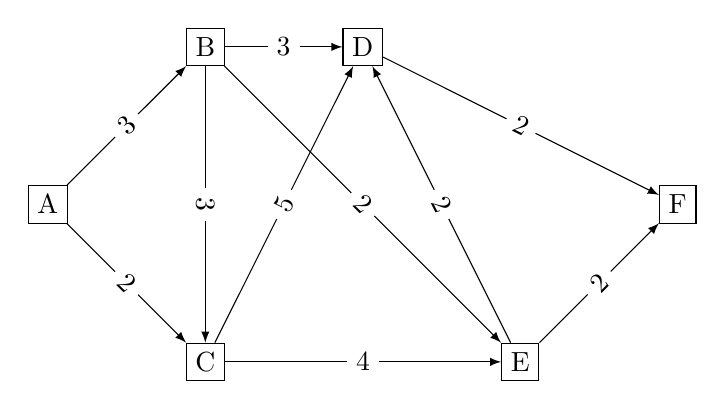
\begin{tikzpicture}
            \node[draw] (A) at (0,0) {A};
            \node[draw] (B) at (2,2) {B};
            \node[draw] (C) at (2,-2) {C};
            \node[draw] (D) at (4,2) {D};
            \node[draw] (E) at (6,-2) {E};
            \node[draw] (F) at (8,0) {F};
    
            \draw[->,>=latex] (A)--(B) node[sloped, midway, fill=white]{3};
            \draw[->,>=latex] (B)--(C) node[sloped, midway, fill=white]{3};
            \draw[->,>=latex] (A)--(C) node[sloped, midway, fill=white]{2};
            \draw[->,>=latex] (B)--(D) node[sloped, midway, fill=white]{3};
            \draw[->,>=latex] (B)--(E) node[sloped, midway, fill=white]{2};
            \draw[->,>=latex] (C)--(D) node[sloped, midway, fill=white]{5};
            \draw[->,>=latex] (C)--(E) node[sloped, midway, fill=white]{4};
            \draw[->,>=latex] (E)--(D) node[sloped, midway, fill=white]{2};
            \draw[->,>=latex] (D)--(F) node[sloped, midway, fill=white]{2};
            \draw[->,>=latex] (E)--(F) node[sloped, midway, fill=white]{2};
    
        \end{tikzpicture}
        \captionof{figure}{graphe orienté et pondéré}
        \label{ospf}
    \end{center}

    \note{\begin{aretenir}[Remarque]
        Les poids de chaque arc représentent le coût de chaque connexion.
    \end{aretenir}
    coût 5 $\rightarrow$ 20Mbit/s\\
    coût 2 $\rightarrow$ 50Mbit/s}
\end{frame}


\subsection{Mise en application}
\begin{frame}[fragile]
    \frametitle{}

    \begin{center}
        \begin{lstlisting}[language=bash, basicstyle=\small, xrightmargin=0.5em, xleftmargin=0.5em]
Créer un tableau des distances entre A et les routeurs (A inclus), initialisées à l'infini.
Dans le tableau modifier la distance vers A à 0.

Tant qu'il reste des routeurs non sélectionnés
    Parmi les routeurs non-sélectionnés, choisir le routeur (noté S) ayant la plus petite distance.
    Pour chaque routeur adjacent à S (noté V) et non déjà sélectionné:
        Si (la distance de V) > (la distance de S + poids S-V)
            La distance de V est remplacée par cette nouvelle valeur
    \end{lstlisting}
        \captionof{code}{Algorithme de Dijkstra}
        \label{dj}
    \end{center}
\note[item]{S = suivant; V = voisin}
\note[item]{ligne 7: on compare encore la distance déjà enregistrée à distance du voisin + arc}
\end{frame}

\begin{frame}
    \frametitle{Initialisation}

    \begin{center}
        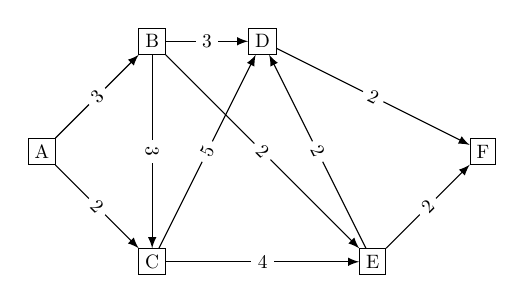
\begin{tikzpicture}[scale=0.7, transform shape]
            \node[draw] (A) at (0,0) {A};
            \node[draw] (B) at (2,2) {B};
            \node[draw] (C) at (2,-2) {C};
            \node[draw] (D) at (4,2) {D};
            \node[draw] (E) at (6,-2) {E};
            \node[draw] (F) at (8,0) {F};
    
            \draw[->,>=latex] (A)--(B) node[sloped, midway, fill=white]{3};
            \draw[->,>=latex] (B)--(C) node[sloped, midway, fill=white]{3};
            \draw[->,>=latex] (A)--(C) node[sloped, midway, fill=white]{2};
            \draw[->,>=latex] (B)--(D) node[sloped, midway, fill=white]{3};
            \draw[->,>=latex] (B)--(E) node[sloped, midway, fill=white]{2};
            \draw[->,>=latex] (C)--(D) node[sloped, midway, fill=white]{5};
            \draw[->,>=latex] (C)--(E) node[sloped, midway, fill=white]{4};
            \draw[->,>=latex] (E)--(D) node[sloped, midway, fill=white]{2};
            \draw[->,>=latex] (D)--(F) node[sloped, midway, fill=white]{2};
            \draw[->,>=latex] (E)--(F) node[sloped, midway, fill=white]{2};
    
        \end{tikzpicture}
    \end{center}
    \begin{center}
        \begin{tabular}{|*{6}{c|}}
            \hline
            A & B      & C      & D      & E      & F      \\
            \hline
            0 & \infty & \infty & \infty & \infty & \infty \\
            \hline
        \end{tabular}
    \end{center}

\end{frame}

\begin{frame}
    \frametitle{Sélection de A}

    \begin{center}
        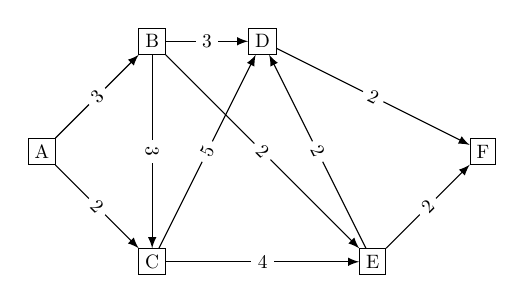
\begin{tikzpicture}[scale=0.7, transform shape]
            \node[draw] (A) at (0,0) {A};
            \node[draw] (B) at (2,2) {B};
            \node[draw] (C) at (2,-2) {C};
            \node[draw] (D) at (4,2) {D};
            \node[draw] (E) at (6,-2) {E};
            \node[draw] (F) at (8,0) {F};
    
            \draw[->,>=latex] (A)--(B) node[sloped, midway, fill=white]{3};
            \draw[->,>=latex] (B)--(C) node[sloped, midway, fill=white]{3};
            \draw[->,>=latex] (A)--(C) node[sloped, midway, fill=white]{2};
            \draw[->,>=latex] (B)--(D) node[sloped, midway, fill=white]{3};
            \draw[->,>=latex] (B)--(E) node[sloped, midway, fill=white]{2};
            \draw[->,>=latex] (C)--(D) node[sloped, midway, fill=white]{5};
            \draw[->,>=latex] (C)--(E) node[sloped, midway, fill=white]{4};
            \draw[->,>=latex] (E)--(D) node[sloped, midway, fill=white]{2};
            \draw[->,>=latex] (D)--(F) node[sloped, midway, fill=white]{2};
            \draw[->,>=latex] (E)--(F) node[sloped, midway, fill=white]{2};
    
        \end{tikzpicture}
    \end{center}
    \begin{center}
        \begin{tabular}{|*{6}{c|}}
            \hline
            A & B & C & D      & E      & F      \\
            \hline
            0 & \textbf{3 (A)} & \textbf{2 (A)} & \infty & \infty & \infty \\
            \hline
        \end{tabular}
        \hspace{2cm}
        \begin{tabular}{|c|}
            \hline
            nœuds visités \\
            \hline
            A             \\
            \hline
        \end{tabular}
    \end{center}

\end{frame}

\begin{frame}
    \frametitle{}

    \begin{activite}
        Continuer de dérouler l'algorithme sur le graphe figure \ref{ospf}.
        \end{activite}

\end{frame}

\begin{frame}
    \frametitle{Correction}

    \begin{center}
        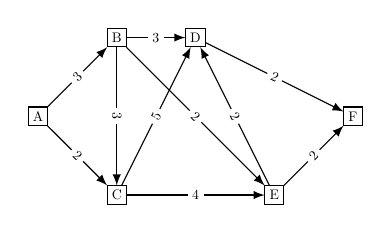
\begin{tikzpicture}[scale=0.5, transform shape]
            \node[draw] (A) at (0,0) {A};
            \node[draw] (B) at (2,2) {B};
            \node[draw] (C) at (2,-2) {C};
            \node[draw] (D) at (4,2) {D};
            \node[draw] (E) at (6,-2) {E};
            \node[draw] (F) at (8,0) {F};
    
            \draw[->,>=latex] (A)--(B) node[sloped, midway, fill=white]{3};
            \draw[->,>=latex] (B)--(C) node[sloped, midway, fill=white]{3};
            \draw[->,>=latex] (A)--(C) node[sloped, midway, fill=white]{2};
            \draw[->,>=latex] (B)--(D) node[sloped, midway, fill=white]{3};
            \draw[->,>=latex] (B)--(E) node[sloped, midway, fill=white]{2};
            \draw[->,>=latex] (C)--(D) node[sloped, midway, fill=white]{5};
            \draw[->,>=latex] (C)--(E) node[sloped, midway, fill=white]{4};
            \draw[->,>=latex] (E)--(D) node[sloped, midway, fill=white]{2};
            \draw[->,>=latex] (D)--(F) node[sloped, midway, fill=white]{2};
            \draw[->,>=latex] (E)--(F) node[sloped, midway, fill=white]{2};
    
        \end{tikzpicture}
    \end{center}
    On sélectionne le nœud non encore visité et avec la plus petite distance: C.
    \begin{center}
        \begin{tabular}{|*{6}{c|}}
            \hline
            A & B & C & D      & E      & F      \\
            \hline
            0 & 3 (A) & 2 (A) & \infty & \infty & \infty \\
            \hline
            \cellcolor{gray} & 3 (A) & 2 (A) & \textbf{7 (C)} & \textbf{6 (C)} & \infty \\
            \hline
        \end{tabular}
        \hspace{2cm}
        \begin{tabular}{|c|}
            \hline
            nœuds visités \\
            \hline
            A - C            \\
            \hline
        \end{tabular}
    \end{center}
\note{cellule grisée = nœud déjà visité, on a déjà sa route la + courte}
\end{frame}

\begin{frame}
    \frametitle{Correction}

    \begin{center}
        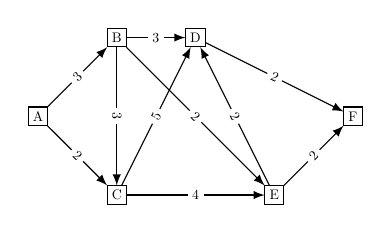
\begin{tikzpicture}[scale=0.5, transform shape]
            \node[draw] (A) at (0,0) {A};
            \node[draw] (B) at (2,2) {B};
            \node[draw] (C) at (2,-2) {C};
            \node[draw] (D) at (4,2) {D};
            \node[draw] (E) at (6,-2) {E};
            \node[draw] (F) at (8,0) {F};
    
            \draw[->,>=latex] (A)--(B) node[sloped, midway, fill=white]{3};
            \draw[->,>=latex] (B)--(C) node[sloped, midway, fill=white]{3};
            \draw[->,>=latex] (A)--(C) node[sloped, midway, fill=white]{2};
            \draw[->,>=latex] (B)--(D) node[sloped, midway, fill=white]{3};
            \draw[->,>=latex] (B)--(E) node[sloped, midway, fill=white]{2};
            \draw[->,>=latex] (C)--(D) node[sloped, midway, fill=white]{5};
            \draw[->,>=latex] (C)--(E) node[sloped, midway, fill=white]{4};
            \draw[->,>=latex] (E)--(D) node[sloped, midway, fill=white]{2};
            \draw[->,>=latex] (D)--(F) node[sloped, midway, fill=white]{2};
            \draw[->,>=latex] (E)--(F) node[sloped, midway, fill=white]{2};
    
        \end{tikzpicture}
    \end{center}
    On sélectionne le nœud non encore visité et avec la plus petite distance: B.
    \begin{center}
        \begin{tabular}{|*{6}{c|}}
            \hline
            A & B & C & D      & E      & F      \\
            \hline
            0 & 3 (A) & 2 (A) & \infty & \infty & \infty \\
            \hline
            \cellcolor{gray} & 3 (A) & 2 (A) & 7 (C) & 6 (C) & \infty \\
            \hline
            \cellcolor{gray} & 3 (A) & \cellcolor{gray} & \textbf{6 (B)} & \textbf{5 (B)} & \infty \\
            \hline
        \end{tabular}
        \hspace{2cm}
        \begin{tabular}{|c|}
            \hline
            nœuds visités \\
            \hline
            A - C - B           \\
            \hline
        \end{tabular}
    \end{center}
\note{C n'est pas regardé: on a déjà trouvé la + petite distance pour lui = il a déjà été visité}
\end{frame}

\begin{frame}
    \frametitle{Correction}

    \begin{center}
        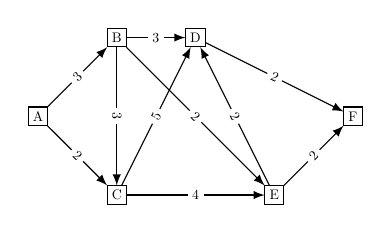
\begin{tikzpicture}[scale=0.5, transform shape]
            \node[draw] (A) at (0,0) {A};
            \node[draw] (B) at (2,2) {B};
            \node[draw] (C) at (2,-2) {C};
            \node[draw] (D) at (4,2) {D};
            \node[draw] (E) at (6,-2) {E};
            \node[draw] (F) at (8,0) {F};
    
            \draw[->,>=latex] (A)--(B) node[sloped, midway, fill=white]{3};
            \draw[->,>=latex] (B)--(C) node[sloped, midway, fill=white]{3};
            \draw[->,>=latex] (A)--(C) node[sloped, midway, fill=white]{2};
            \draw[->,>=latex] (B)--(D) node[sloped, midway, fill=white]{3};
            \draw[->,>=latex] (B)--(E) node[sloped, midway, fill=white]{2};
            \draw[->,>=latex] (C)--(D) node[sloped, midway, fill=white]{5};
            \draw[->,>=latex] (C)--(E) node[sloped, midway, fill=white]{4};
            \draw[->,>=latex] (E)--(D) node[sloped, midway, fill=white]{2};
            \draw[->,>=latex] (D)--(F) node[sloped, midway, fill=white]{2};
            \draw[->,>=latex] (E)--(F) node[sloped, midway, fill=white]{2};
    
        \end{tikzpicture}
    \end{center}
    On sélectionne le nœud non encore visité et avec la plus petite distance: E.
    \begin{center}
        \begin{tabular}{|*{6}{c|}}
            \hline
            A & B & C & D      & E      & F      \\
            \hline
            0 & 3 (A) & 2 (A) & \infty & \infty & \infty \\
            \hline
            \cellcolor{gray} & 3 (A) & 2 (A) & 7 (C) & 6 (C) & \infty \\
            \hline
            \cellcolor{gray} & 3 (A) & \cellcolor{gray} & 6 (B) & 5 (B) & \infty \\
            \hline
            \cellcolor{gray} & \cellcolor{gray} & \cellcolor{gray} & 6 (B) & 5 (B) & \textbf{7 (E)} \\
            \hline
        \end{tabular}
        \hspace{2cm}
        \begin{tabular}{|c|}
            \hline
            nœuds visités \\
            \hline
            A - C - B - E    \\
            \hline
        \end{tabular}
    \end{center}

\end{frame}

\begin{frame}
    \frametitle{Correction}

    \begin{center}
        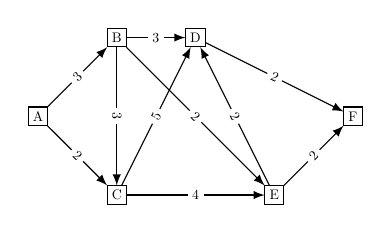
\begin{tikzpicture}[scale=0.5, transform shape]
            \node[draw] (A) at (0,0) {A};
            \node[draw] (B) at (2,2) {B};
            \node[draw] (C) at (2,-2) {C};
            \node[draw] (D) at (4,2) {D};
            \node[draw] (E) at (6,-2) {E};
            \node[draw] (F) at (8,0) {F};
    
            \draw[->,>=latex] (A)--(B) node[sloped, midway, fill=white]{3};
            \draw[->,>=latex] (B)--(C) node[sloped, midway, fill=white]{3};
            \draw[->,>=latex] (A)--(C) node[sloped, midway, fill=white]{2};
            \draw[->,>=latex] (B)--(D) node[sloped, midway, fill=white]{3};
            \draw[->,>=latex] (B)--(E) node[sloped, midway, fill=white]{2};
            \draw[->,>=latex] (C)--(D) node[sloped, midway, fill=white]{5};
            \draw[->,>=latex] (C)--(E) node[sloped, midway, fill=white]{4};
            \draw[->,>=latex] (E)--(D) node[sloped, midway, fill=white]{2};
            \draw[->,>=latex] (D)--(F) node[sloped, midway, fill=white]{2};
            \draw[->,>=latex] (E)--(F) node[sloped, midway, fill=white]{2};
    
        \end{tikzpicture}
    \end{center}
    On sélectionne le nœud non encore visité et avec la plus petite distance: D.
    \begin{center}
        \begin{tabular}{|*{6}{c|}}
            \hline
            A & B & C & D      & E      & F      \\
            \hline
            0 & 3 (A) & 2 (A) & \infty & \infty & \infty \\
            \hline
            \cellcolor{gray} & 3 (A) & 2 (A) & 7 (C) & 6 (C) & \infty \\
            \hline
            \cellcolor{gray} & 3 (A) & \cellcolor{gray} & 6 (B) & 5 (B) & \infty \\
            \hline
            \cellcolor{gray} & \cellcolor{gray} & \cellcolor{gray} & 6 (B) & 5 (B) & 7 (E) \\
            \hline
            \cellcolor{gray} & \cellcolor{gray} & \cellcolor{gray} & 6 (B) & \cellcolor{gray} & 7 (E) \\
            \hline
        \end{tabular}
        \hspace{2cm}
        \begin{tabular}{|c|}
            \hline
            nœuds visités \\
            \hline
            A - C - B - E - D   \\
            \hline
        \end{tabular}
    \end{center}
\note{pas de modification}
\end{frame}

\begin{frame}
    \frametitle{Correction}

    \begin{center}
        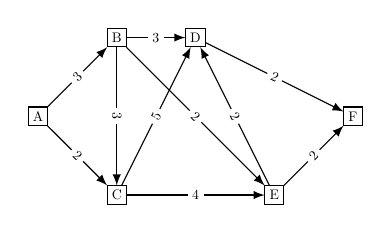
\begin{tikzpicture}[scale=0.5, transform shape]
            \node[draw] (A) at (0,0) {A};
            \node[draw] (B) at (2,2) {B};
            \node[draw] (C) at (2,-2) {C};
            \node[draw] (D) at (4,2) {D};
            \node[draw] (E) at (6,-2) {E};
            \node[draw] (F) at (8,0) {F};
    
            \draw[->,>=latex] (A)--(B) node[sloped, midway, fill=white]{3};
            \draw[->,>=latex] (B)--(C) node[sloped, midway, fill=white]{3};
            \draw[->,>=latex] (A)--(C) node[sloped, midway, fill=white]{2};
            \draw[->,>=latex] (B)--(D) node[sloped, midway, fill=white]{3};
            \draw[->,>=latex] (B)--(E) node[sloped, midway, fill=white]{2};
            \draw[->,>=latex] (C)--(D) node[sloped, midway, fill=white]{5};
            \draw[->,>=latex] (C)--(E) node[sloped, midway, fill=white]{4};
            \draw[->,>=latex] (E)--(D) node[sloped, midway, fill=white]{2};
            \draw[->,>=latex] (D)--(F) node[sloped, midway, fill=white]{2};
            \draw[->,>=latex] (E)--(F) node[sloped, midway, fill=white]{2};
    
        \end{tikzpicture}
    \end{center}
    On sélectionne le nœud non encore visité et avec la plus petite distance: F.
    \begin{center}
        \begin{tabular}{|*{6}{c|}}
            \hline
            A & B & C & D      & E      & F      \\
            \hline
            0 & 3 (A) & 2 (A) & \infty & \infty & \infty \\
            \hline
            \cellcolor{gray} & 3 (A) & 2 (A) & 7 (C) & 6 (C) & \infty \\
            \hline
            \cellcolor{gray} & 3 (A) & \cellcolor{gray} & 6 (B) & 5 (B) & \infty \\
            \hline
            \cellcolor{gray} & \cellcolor{gray} & \cellcolor{gray} & 6 (B) & 5 (B) & 7 (E) \\
            \hline
            \cellcolor{gray} & \cellcolor{gray} & \cellcolor{gray} & 6 (B) & \cellcolor{gray} & 7 (E) \\
            \hline
            \cellcolor{gray} & \cellcolor{gray} & \cellcolor{gray} & \cellcolor{gray} & \cellcolor{gray} & 7 (E)\\
            \hline
        \end{tabular}
        \hspace{2cm}
        \begin{tabular}{|c|}
            \hline
            nœuds visités \\
            \hline
            A - C - B - E - D - F  \\
            \hline
        \end{tabular}
    \end{center}
\note{pas de modification}
\end{frame}

\begin{frame}
    \frametitle{Correction}

    \begin{center}
        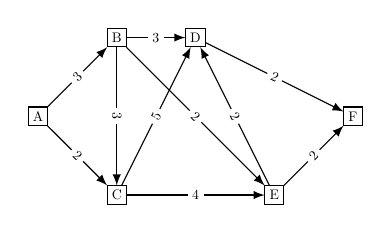
\begin{tikzpicture}[scale=0.5, transform shape]
            \node[draw] (A) at (0,0) {A};
            \node[draw] (B) at (2,2) {B};
            \node[draw] (C) at (2,-2) {C};
            \node[draw] (D) at (4,2) {D};
            \node[draw] (E) at (6,-2) {E};
            \node[draw] (F) at (8,0) {F};
    
            \draw[->,>=latex] (A)--(B) node[sloped, midway, fill=white]{3};
            \draw[->,>=latex] (B)--(C) node[sloped, midway, fill=white]{3};
            \draw[->,>=latex] (A)--(C) node[sloped, midway, fill=white]{2};
            \draw[->,>=latex] (B)--(D) node[sloped, midway, fill=white]{3};
            \draw[->,>=latex] (B)--(E) node[sloped, midway, fill=white]{2};
            \draw[->,>=latex] (C)--(D) node[sloped, midway, fill=white]{5};
            \draw[->,>=latex] (C)--(E) node[sloped, midway, fill=white]{4};
            \draw[->,>=latex] (E)--(D) node[sloped, midway, fill=white]{2};
            \draw[->,>=latex] (D)--(F) node[sloped, midway, fill=white]{2};
            \draw[->,>=latex] (E)--(F) node[sloped, midway, fill=white]{2};
    
        \end{tikzpicture}
    \end{center}
    On sélectionne le nœud non encore visité et avec la plus petite distance: F.
    \begin{center}
        \begin{tabular}{|*{6}{c|}}
            \hline
            A & B & C & D      & E      & F      \\
            \hline
            0 & 3 (A) & 2 (A) & \infty & \infty & \infty \\
            \hline
            \cellcolor{gray} & 3 (A) & 2 (A) & 7 (C) & 6 (C) & \infty \\
            \hline
            \cellcolor{gray} & 3 (A) & \cellcolor{gray} & 6 (B) & 5 (B) & \infty \\
            \hline
            \cellcolor{gray} & \cellcolor{gray} & \cellcolor{gray} & 6 (B) & 5 (B) & 7 (E) \\
            \hline
            \cellcolor{gray} & \cellcolor{gray} & \cellcolor{gray} & 6 (B) & \cellcolor{gray} & 7 (E) \\
            \hline
            \cellcolor{gray} & \cellcolor{gray} & \cellcolor{gray} & \cellcolor{gray} & \cellcolor{gray} & 7 (E) \\
            \hline
            \cellcolor{gray} & \cellcolor{gray} & \cellcolor{gray} & \cellcolor{gray} & \cellcolor{gray} & \cellcolor{gray} \\
            \hline
        \end{tabular}
        \hspace{2cm}
        \begin{tabular}{|c|}
            \hline
            nœuds visités \\
            \hline
            A - C - B - E - D - F  \\
            \hline
        \end{tabular}
    \end{center}
\note{tous les nœuds ont été visités = fin de l'algorithme. On peut reconstruire le chemin.\\
pour F: F $\rightarrow$ E $\rightarrow$ B $\rightarrow$ A}
\end{frame}

\subsection{Complexité}
\begin{frame}[fragile]
    \frametitle{}

    \begin{itemize}
        \item<1->La complexité dépend du nombre de sommets S et du nombre d'arcs A.
        \item<2->Le point clé de l'algorithme tient dans la recherche de la distance minimale.
        \begin{center}
        \begin{lstlisting}[language=bash, basicstyle=\small, xleftmargin=0.5em, xrightmargin=0.5em]
Parmi les routeurs non-sélectionnés, choisir le routeur (noté S) ayant la plus petite distance.        
        \end{lstlisting}
        \end{center}
    \end{itemize}
\note[item]{hors programme}
\note[item]{utilisation de tas par exemple}
\end{frame}

\begin{frame}
    \frametitle{Complexité de l'algorithme de Dijkstra}

    {\LARGE $$O((A+S)×\log{S})$$    }

\end{frame}
\end{document}